\section{Fault Recurrence from Geology}

The second set of tools is designed to support a workflow in which the modeller has sufficient information to define both the geometry of the active fault surface and the slip rate, from which they then wish to calculate the activity rate on the fault according to a particular magnitude frequency distribution. It is recognised that in practice this is a complex and challenging process as the physical parameters of many faults may be highly uncertain, and the propagation of this uncertainty is critical in defining the epistemic uncertainty on such source models \parencite{Peruzza_etal2010}. The current implementation of the tools focusses on the time-independent workflow entirely, aiming to allow the user to constrain the activity rate from the geological slip for an assumed single section. It is hoped that in future this will evolve to consider more complex conditions, such as those in which the observations of displacement at points along the segment and interactions between segments can be taken into consideration. The manner in which these features take shape will become clearer as more data is input into the global fault database created by the GEM Faulted Earth project.

The core of the time-independent workflow originates from the simple moment balance 
in which the total moment release rate (in Nm) on the fault $\dot{M}_o$ is derived from the slip rate $\dot{s}$\parencite{AndersonLuco1983, Bungum2007}: 

\begin{equation}
\dot{M}_o = c \mu A \dot{s}
\end{equation}

where A is the area of the fault surface (in $km^2$), $\mu$ is the shear modulus (characterised in the toolkit in terms of GigaPascals, GPa) and $c$ the coefficient of seismogenic coupling. Slip rates must be input in $mm\ yr^{-1}$; lengths and area in $km$ or $km^2$ respectively. The magnitude frequency distribution calculators differ primarily in the manner in which this moment rate is distributed in order to constrain the activity rate. The different calculators are described below.

\subsection{Epistemic Uncertainties in the Fault Modelling}

The manner in which epistemic uncertainties are incorporated into the fault recurrence calculation would appear to vary somewhat in practice. This is in no small part due to the manner in which the uncertainty on the contributing parameters is represented in a quantitative sense. For the present implementation, and driven in part by the need for consistency with the OpenQuake hazardlib, a purely decision based epistemic uncertainty analysis is supported. This requires that, for each parameter upon which epistemic uncertainty is supported, the user must specify the alternative values and the corresponding weightings. Currently, we support epistemic uncertainty on six different parts of the model:

\begin{enumerate}
\item Slip Rate ($mm\ yr^{-1}$)

\item Magnitude Scaling Relation

\item Shear Modulus ($GPa$)

\item Displacement to Length Ratio

\item Number of standard deviations on the Magnitude Scaling Relation

\item Configuration of the Magnitude Frequency Distribution
\end{enumerate}

As input to the function, these epistemic uncertainties must be represented as a list of tuples, with a corresponding value and weight. For example, if one wished to characterise the slip on a fault by three values (e.g. 3.0, 5.0, 7.0) with corresponding weightings (e.g. 0.25, 0.5, 0.25), the slip should be defined as shown below: 

\begin{python}[frame=single]
>> slip = [(3.0, 0.25), (5.0, 0.5), (7.0, 0.25)]
\end{python}

In characterising uncertainty in this manner the user is essentially creating a logic tree for each source, in which the total number of activity rate models (i.e. the end branches of the logic tree) is the product of the number of alternative values input for each supported parameter. The user can make a choice as to how they wish this uncertainty to be represented in the resulting hazard model:

\subsubsection{Complete Enumeration}

This will essentially reproduce the fault in the source model N times, where N is the total number of end branches, where on each branch the resulting activity rate is multiplied by the end weight the branch.

\subsubsection{Collapsed Branches}

In some cases it may become to costly to reproduce faults models separately for each end branch, and the user may simply wish to collapse the logic tree into a single activity rate. This rate, represented by an incremental magnitude frequency distribution, is the sum of the weighted activity rates on all the branches. To calculate this the program will determine the minimum and maximum magnitude of all the branches, then using a user specified bin width will calculate the weighted sum of the occurrence rates in each bin. 

N.B. When collapsing the branches it the original magnitude scaling relations used on the branches and the scaling relation associated to the source in the resulting OpenQuake source model are not necessarily the same! The user will need to specify the scaling relation that will be assigned to the fault source when the branches are collapsed. 

\subsubsection{Magnitude Scaling Relations}

To ensure compatibility with the OpenQuake engine, the scaling relations are taken directly from the OpenQuake library. Therefore the only scaling relations available are those that can be currently found in the oq-hazardlib (\textcite{wells1994} and \textcite{thomas2010} at the time of writing). To implement new magnitude scaling relations the reader is referred to the documentation and source code for the OpenQuake hazard library (\href{http://docs.openquake.org/oq-hazardlib}{http://docs.openquake.org/oq-hazardlib})

\subsection{Tectonic Regionalisation}

Recognising once again that certain parameters may not be possible to constrain on a fault by fault basis, a tectonic regionalisation can be invoked in order to define parameters, or a distribution of values, that can be assigned to all faults sharing that tectonic regionalisation classification. At present, the regionalisation can be used to define default parameters/distributions for:

\begin{enumerate}
\item Magnitude Scaling Relation
\item Shear Modulus
\item Displacement to Length Ratio
\end{enumerate}

If defining a tectonic regionalisation the inputs must be specified as a set of tuples, in the same fashion as described for the epistemic uncertainties. In the present version there is no direct geographical link between the fault and the tectonic region (i.e. the regionalisation is a data holder and does not have geographical attributes), although it is anticipated that this may change in the future. At present it will be necessary to indicate for each fault the tectonic regionalisation class to which it belongs.


%The second exercise in this demonstration considers how information from geology can be used to define seismogenic source models for Simple and/or Complex Fault typologies supported by OpenQuake. Here, we consider the Himalayan Main Boundary Thrust (MBT), which has been divided into three sections (segments): western, central, eastern. 
%
%The geometry of the three segments of the MBT are derived from the fault database of \cite{TaylorYin2009} with slip rates of $25 mm\ yr^-1$, $20.0 mm\ yr^1$, and $18.0 mm\ yr^1$ assigned to the western, central and eastern segments respectively. Seismogenic coupling is assumed to a depth of 25 km, whilst the coupling coefficient itself is 1.0 (i.e. fully coupled).
%
%For the examples shown we consider only a single characteristic earthquake, with uncertainty represented via a Gaussian distribution truncated at -3 and 3 standard deviations ($\sigma$), with the standard deviation equal to 0.12 magnitude units. The magnitude scaling relation used in this example is \cite{wells1994}. 

\subsection{Definition of the Fault Input}

\subsubsection{The ``YAML'' Format}

The establishment of a standard xml for representing input faults in OpenQuake remains to be undertaken, and will be done so following the completion of the GEM Faulted Earth project. The current version supports a less verbose, and more human-readable, characterisation using the ``Yet Another Markup Language (YAML)'' format. The Yaml format is both case and spacing sensitive, so care must be paid to the spacing and the punctuation characters below. For development, the primary advantage of the Yaml format
is that the data are largely being defined in a manner that is consistent with the 
corresponding python objects, lists and dictionaries. This makes the reading of the file a simpler process. 

A template example (for a single simple fault) is broken down into steps below.

The first component of the Yaml file is the tectonic regionalisation:

\begin{Verbatim}[frame=single, commandchars=\\\{\}, fontsize=\scriptsize]
\#*****************************************************************************
\#FAULT FILE IN YAML (Yet Another Markup Language) FORMAT
\#*****************************************************************************
\#
tectonic_regionalisation:
    - Name: Active Shallow Crust
      Code: 001
      \# Magnitude scaling relation (see http://docs.openquake.org/oq-hazardlib)
      \#for currently available choices!
      Magnitude_Scaling_Relation: \{
          Value: [WC1994],
          Weight: [1.0]\}
      \# Shear Modulus (in gigapascals, GPa)
      Shear_Modulus: \{
          Value: [30.0],
          Weight: [1.0]\}
      \# Fault displacement to length ratio
      Displacement_Length_Ratio: \{
          Value: [1.25E-5],
          Weight: [1.0]\}
\end{Verbatim}

Here the tectonic regionalisation represents a list of categories (albeit only one is shown above). The lists elements are demarcated by the ( - ) symbol and all indentation is with respect to that symbol. So in the above example, a single region class has been defined with the name ``Active Shallow Crust'' and a unique identifier code ``001''. The default values are now provided for the three data attributes: magnitude scaling relation, shear modulus and displacement to length ratio. Each attribute is associated with a dictionary containing two keys: ``Value'' and ``Weight'', which then define the lists of the values and the corresponding weights, respectively.

N.B. If, for any of the above attributes, the number of weights is not the same as the number of values, or the weights do not sum to 1.0 then an error will be raised! 

A fault model must be defined with both a model identifier key (``001'') and a model name, ``001'' and ``Template Simple Fault'' in the example below. From then on the each fault is then defined as an element in the list.
       
\begin{Verbatim}[frame=single, commandchars=\\\{\}, fontsize=\scriptsize]
Fault_Model_ID: 001
Fault_Model_Name: Template Simple Fault
Fault_Model:
    - ID: 001
      Tectonic_Region: Active Shallow Crust
      Fault_Name: A Simple Fault
      Fault_Geometry: \{
          Fault_Typology: Simple,
          \# For simple typology, defines the trace in terms of Long., Lat.
          Fault_Trace: [30.0, 30.0,
                        30.0, 31.5],

          \# Upper Seismogenic Depth (km)
          Upper_Depth: 0.0,
          \# Lower Seismogenic Depth (km)
          Lower_Depth: 20.0,
          Strike: ,
          \# Dip (degrees)
          Dip: 60.\}
      Rake: -90
      Slip_Type: Thrust
      Slip_Completeness_Factor: 1
      \# slip [value_1, value_2, ... value_n]
      \# [weight_1, weight_2, ... weight_n]
      Slip: \{
          Value: [18., 20.0, 23.],
          Weight: [0.3, 0.5, 0.2]\}
      \#Aseismic Slip Factor
      Aseismic: 0.0
      MFD_Model:
          \# Example of constructor for characteristic earthquake
        - Model_Type: Characteristic
          \# Spacing (magnitude units) of the magnitude frequency distribution
          MFD_spacing: 0.1
          \# Weight of the model
          Model_Weight: 0.2
          \# Magnitude of the Characteristic Earthquake
          Maximum_Magnitude:
          \# Uncertainty on Characteristic Magnitude (in magnitude units)
          Sigma: 0.12
          \# Lower bound truncation (in number of standard deviations)
          Lower_Bound: -3.0
          \# Upper bound truncation (in number of standard deviations)
          Upper_Bound: 3.0
          \####################################################
        - Model_Name: AndersonLucoArbitrary
          \# Example constructor of the Anderson & Luco (1983) - Arbitrary Exponential
          \# Type - chooses between type 1 ('First'), type 2 ('Second') or type 3 ('Third')
          Type: First
          MFD_spacing: 0.1
          Model_Weight: 0.1
          \# Maximum Magnitude of the exponential distribution
          Maximum_Magnitude:
          Maximum_Magnitude_Uncertainty:
          Minimum_Magnitude: 4.5
          \# b-value of the exponential distribution as [expected, uncertainty]
          b_value: [0.8, 0.05]
          \####################################################
        - Model_Name: AndersonLucoAreaMmax
          \# Example constructor of the Anderson & Luco (1983) - Area-Mmax Exponential
          \# Type - chooses between type 1 ('First'), type 2 ('Second') or type 3 ('Third')
          Model_Type: Second
          MFD_spacing: 0.1
          Model_Weight: 0.1
          Maximum_Magnitude:
          Maximum_Magnitude_Uncertainty:
          Minimum_Magnitude: 4.5
          b_value: [0.8, 0.05]
          \####################################################
        - Model_Name: YoungsCoppersmithExponential
          \# Example constructor of the Youngs & Coppersmith (1985) Exponential model
          MFD_spacing: 0.1
          Model_Weight: 0.3
          Maximum_Magnitude:
          Maximum_Magnitude_Uncertainty:
          Minimum_Magnitude: 5.0
          b_value: [0.8, 0.05]
          ####################################################
          \# Example constructor of the Youngs & Coppersmith (1985) Characteristic model
        - Model_Name: YoungsCoppersmithCharacteristic
          Model_Weight: 0.3
          Maximum_Magnitude:
          Maximum_Magnitude_Uncertainty:
          Minimum_Magnitude: 5.0
          MFD_spacing: 0.1
          b_value: [0.8, None]
      Shear_Modulus: \{
          Value: [30., 35.0],
          Weight: [0.8, 0.2]\}
      Magnitude_Scaling_Relation: \{
          Value: [WC1994],
          Weight: [1.0]\}
      Scaling_Relation_Sigma: \{
          Value: [-1.5, 0.0, 1.5],
          Weight: [0.15, 0.7, 0.15]\}
      Aspect_Ratio: 1.5
      Displacement_Length_Ratio: \{
          Value: [1.25E-5, 1.5E-5],
          Weight:[0.5, 0.5]\}
\end{Verbatim}

The details of the magnitude frequency distribution configurations \verb=MFD_Model= will be expanded upon in the respective sections. The critical attributes for a fault are then:

\begin{itemize}
\item \verb=ID= The unique identifier for the fault
\item \verb=Name= The fault name
\item \verb=Tectonic Region= The tectonic region class to which the fault is assigned. Note that if the region class if not defined in the tectonic region header than an error will be raised.
\item \verb=Fault Geometry= A dictionary of the geometrical properties of the fault (described in further detail in due course
\item \verb=Rake= The rake of the fault (as defined using the \textcite{aki2002} convention)
\item \verb=Slip= A dictionary with the slip rate of the fault in mm yr$^{-1}$ and their corresponding uncertainties
\item \verb=Aseismic= A coefficient describing the pfraction of slip released aseismically (effectively $1 - c$ where $c$ is the coupling coefficient)
\item \verb=MFD_Model= A list of models describing the corresponding magnitude frequency distribution properties
\item \verb=Aspect_Ratio= The rupture aspect ratio
\item \verb=Scaling_Relation_Sigma= The number of standard deviations of the magnitude scaling relation and their corresponding weights. 
\end{itemize}

For shear modulus, magnitude scaling relation and displacement to length ratio the fault input is the same as for the tectonic regionalisation. These attributes can be for a single fault, but if they are not provided for the fault they can be defined within the tectonic regionalisation. If they are not defined within the tectonic regionalisation then the default values are assumed: 30 GPa for the shear modulus, \textcite{wells1994} for the scaling relation and $1.25\times10^{-5}$ for the displacement to length ratio. 

The remaining attributes are not essential and are not used in the calculation at present, but are included for completeness:
\begin{itemize}
\item \verb=Slip_Type= Description of the type of slip (i.e. normal, thrust, etc.)
\item \verb=Slip_Completeness_Factor= The completeness factor (or quality factor) of the slip as an integer from 1 (Well constrained) to 4 (Unconstrained) 
\end{itemize}


\subsection{Fault Recurrence Models}

The current implementation of the hmtk supports nine different models for deriving recurrence models from geological parameters. Six different models are provided for exponential distributions, which originate from the study of \textcite{AndersonLuco1983}, one for a ''simple characteristic'' earthquake (used here), a further exponential model \parencite{YoungsCoppersmith1985} and the hybrid characteristic-exponential model also presented by \textcite{YoungsCoppersmith1985}. Models describing exponential recurrence requiring the definition of a ''b-value'' for each source. The various nuances and assumptions behind each model are described in the sources cited here, and the reader is strongly encouraged to refer to the source material for further detail.

Common to many of these models is the moment magnitude definition of \textcite{HanksKanamori1979}:

\begin{equation}
M_o \left( {M_W} \right) = 10.0 ^{16.05 + 1.5 M_W} = M_o \left( {M_{MAX}} \right) e^{-\bar{d} \Delta M}
\end{equation}

where $\bar{d} = 1.5 \log_e \left( {10.0} \right)$.

\subsubsection{\textcite{AndersonLuco1983} ``Arbitrary''}

The study of \textcite{AndersonLuco1983} defines three categories of models for defining a magnitude recurrence distribution from the geological slip. The first model refers to the case when the recurrence is related to the entire fault, which we call the ``Arbitrary`` model here. The second model refers the recurrence to the rupture area of the maximum earthquake, the ``Area Mmax'' model here. The third category relates the recurrence to a specific site on the fault, and is not yet implemented in to tools. From within each of the three categories there are three different subcategories, which allow for different forms of tapering at the upper edge of the model. The reader is referred to the original paper of \textcite{AndersonLuco1983} for further details and a complete derivation of the models. The different forms of the recurrence model are referred to here as types 1, 2 and 3, which correspond to equations 4, 3 and 2 in the original paper of \textcite{AndersonLuco1983}. 

\begin{enumerate}
\item The `first' type of \textcite{AndersonLuco1983} arbitrary model is defined as:
\begin{equation}
N \left( {M_W \geq M} \right) = \frac{\bar{d} - \bar{b}}{\bar{d}} \frac{\mu A \dot{s}}{M_o \left( {M_{MAX}} \right)} \exp \left( {\bar{b} \left[ {M_{MAX} - M} \right]} \right)
\end{equation}

where $\bar{b} = b \log_e \left( {10.0} \right)$, $M_o \left( {M_{MAX}} \right)$ is the moment of the maximum magnitude, and $A$ and $\dot{s}$ are the are of the fault and the slip rate, as defined previously.

\item The `second' type of model is defined as:
\begin{equation}
N \left( {M_W \geq M} \right) = \frac{\bar{d} - \bar{b}}{\bar{b}} \frac{\mu A \dot{s}}{M_o \left( {M_{MAX}} \right)} \exp \left( {-\bar{b} \left[ {M_{MAX} - M} \right] - 1} \right)
\end{equation}

\item The `third' type of model is defined as:
\begin{equation}\begin{split}
N \left( {M_W \geq M} \right) = & \frac{\bar{d} \left( {\bar{d} - \bar{b}} \right)}{\bar{b}} \frac{\mu A \dot{s}}{M_o \left( {M_{MAX}} \right)} \times \ldots \\
&\left( {\frac{1}{\bar{b}} \left( {\exp \left( {\bar{b} \left[ {M_{MAX} - M} \right]} \right) - 1} \right)  - \left[ {M_{MAX} - M} \right]} \right)
\end{split}\end{equation}
\end{enumerate}

The configuration of the \verb=MFD_Model= for the \textcite{AndersonLuco1983} ``Arbitrary'' calculators shown as follows:

\begin{Verbatim}[frame=single, commandchars=\\\{\}, fontsize=\scriptsize]
        - Model_Name: AndersonLucoArbitrary
          \# Example constructor of the Anderson & Luco (1983) - Arbitrary Exponential
          \# Type - chooses between type 1 ('First'), type 2 ('Second') or type 3 ('Third')
          Type: First
          MFD_spacing: 0.1
          Model_Weight: 0.1
          \# Maximum Magnitude of the exponential distribution
          Maximum_Magnitude:
          Maximum_Magnitude_Uncertainty:
          Minimum_Magnitude: 4.5
          \# b-value of the exponential distribution as [expected, uncertainty]
          b_value: [0.8, 0.05]
\end{Verbatim}

The \verb=Model_Name= and the \verb=Type= are self explanatory. \verb=Model_Weight= is the weighting of the particular MFD within the epistemic uncertainty analysis. \verb=MFD_Spacing= is the spacing of the evenly discretized magnitude frequency distribution that will be output. The three parameters \verb=Minimum_Magnitude=, \verb=Maximum_Magnitude= and \\ \verb=Maximum_Magnitude_Uncertainty= define the bounding limits of the MFD and the standard deviation of $M_{MAX}$ in $M_W$ units. \verb=Minimum_Magnitude= is an essential attribute, whereas \verb=Maximum_Magnitude= and \verb=Maximum_Magnitude_Uncertainty= are optional. If not specified the code will calculate \verb=Maximum_Magnitude= and \\ \verb=Maximum_Magnitude_Uncertainty= from the magnitude scaling relationship. Finally, as these are exponential models the b-value must be specified. Here it is preferred that b-value is specified as a tuple of $\left[ {b-value, b-value\ error} \right]$, although at present the epistemic uncertainty on b-value does not propagate (this may change in future!). 

As with the catalogue tools, plotting functions are available to assist the user understand the nature of the recurrence model used for a given fault. To illustrate the impact of the choice of the `first', `second' and `third' type of model we consider a simple fault with the following properties: along-strike length = 200 km, down-dip width = 20 km, rake = 0.0 (strike-slip) and slip-rate = 10 mm/yr. The \textcite{wells1994} magnitude scaling relation is assumed. The fault and three magnitude frequency distributions are configured as shown:

\begin{python}[frame=single]
>> slip = 10.0  # Slip rate in mm/yr
# Area = along-strike length (km) * down-dip with (km)
>> area = 100.0 * 20.0
# Rake = 0.
>> rake = 0.
\# Magnitude Scaling Relation
>> from openquake.hazardlib.scalerel.wc1994 import WC1994
>> msr = WC1994()

>> and_luc_config1 = {'Model_Name':'AndersonLucoArbitrary',
                      'Model_Type': 'First',
                      'Model_Weight': 1.0,  
                      'MFD_spacing': 0.1,
                      'Maximum_Magnitude': None,
                      'Minimum_Magnitude': 4.5,
                      'b_value': [0.8, 0.05]}
>> and_luc_config2 = {'Model_Name': 'AndersonLucoArbitrary',
                      'Model_Type': 'Second',
                      'Model_Weight': 1.0,
                      'MFD_spacing': 0.1,
                      'Maximum_Magnitude': None,
                      'Minimum_Magnitude': 4.5,
                      'b_value': [0.8, 0.05]}
>> and_luc_config3 = {'Model_Name': 'AndersonLucoArbitrary',
                      'Model_Type': 'Third',
                      'Model_Weight': 1.0,   
                      'MFD_spacing': 0.1,
                      'Maximum_Magnitude': None,
                      'Minimum_Magnitude': 4.5,
                      'b_value': [0.8, 0.05]}
\end{python}
\begin{figure}[htb]
  \centering
      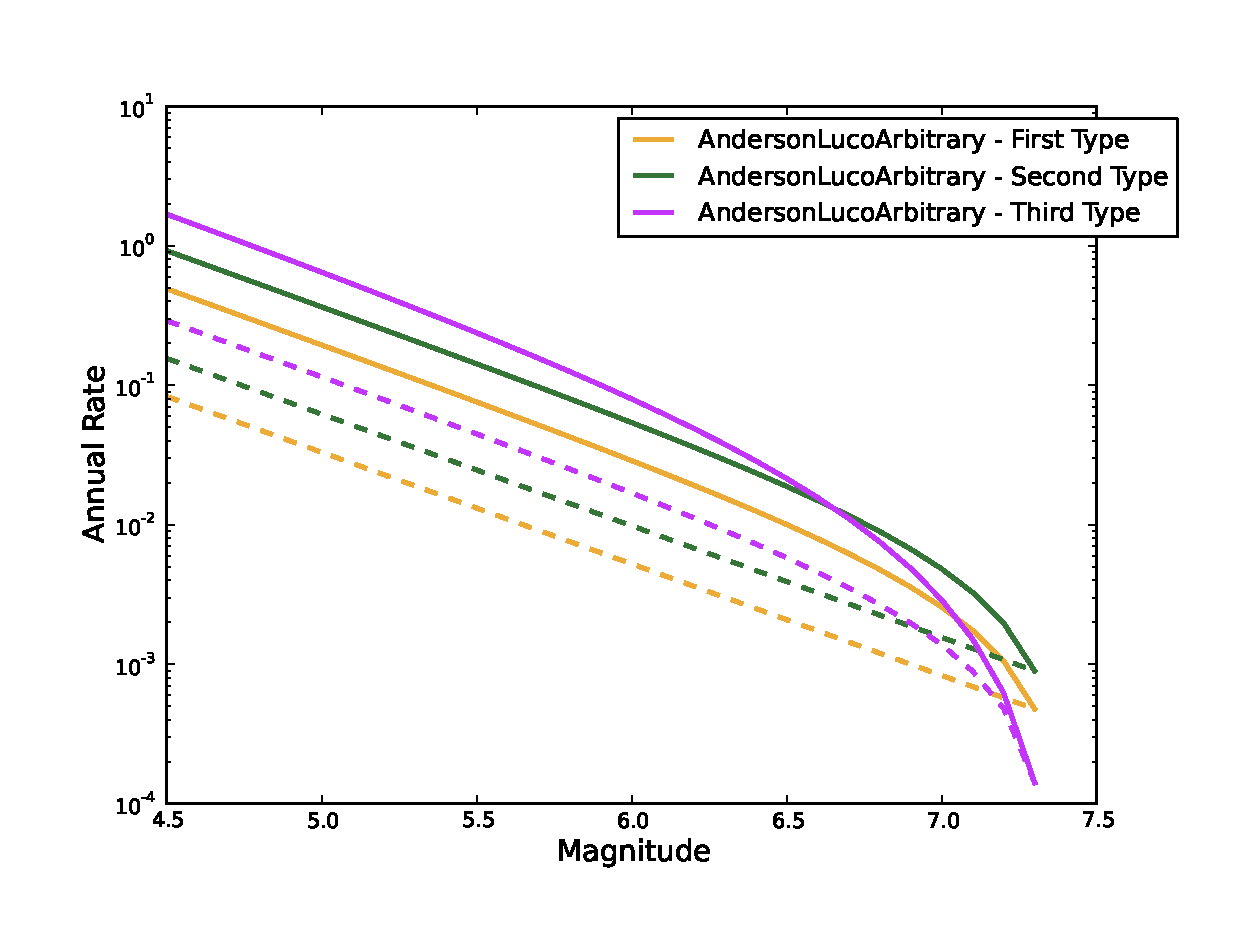
\includegraphics[trim=5mm 5mm 5mm 5mm, clip, width=12cm]{./figures/anderson_luco_arbitrary_mfds.eps}
  \caption{Comparison of magnitude frequency distributions for the specified fault using the three different models of the \cite{AndersonLuco1983} ``Arbitrary'' configuration}
  \label{fig:anderson_luco_arb}
\end{figure}
The models are then compared, as shown in Figure \ref{fig:anderson_luco_arb}, using the following commands:

\begin{python}[frame=single]
>> anderson_luco_arb = [and_luc_config1,
                        and_luc_config2,
                        and_luc_config3]
# Import geological recurrence model plotting function
>> from hmtk.plotting.faults.geology_mfd_plot import\
     plot_recurrence_models
>> plot_recurrence_models(anderson_luco_arb,
                          area,
                          slip,
                          msr,
                          rake,
                          msr_sigma=0.0) # Number of standard 
                                         # deviations above or
                                         # below the median msr 
\end{python}



\subsubsection{\textcite{AndersonLuco1983} ``Area Mmax''}

The second set of models from \textcite{AndersonLuco1983} consider the case when the the recurrence model is referred to the rupture area of the maximum earthquake specified on the fault. As the area is not extracted directly from the geometry, additional information must be provided, namely the aspect ratio of ruptures on the fault and the displacement to length ratio ($\alpha$) of the fault \parencite{Bungum2007}. This information is used to derived an additional parameter ($\beta$):

\begin{equation}
\beta=\sqrt{\frac{\alpha M_o \left( 0 \right)}{\mu W}}
\end{equation}

The three types of \textcite{AndersonLuco1983} ``Area Mmax'' model are then calculated via:

\begin{enumerate}

\item Type 1 (``First'')

\begin{equation}
N \left( {M_W \geq M} \right) = \frac{\bar{d} - \bar{b}}{\bar{d}} \frac{\dot{s}}{\beta} \exp \left( {-\frac{\bar{d}}{2} M_{MAX}} \right) \exp \left( {\bar{b} \left[ {M_{MAX} - M} \right]} \right)
\end{equation}


\item Type 2 (``Second'')

\begin{equation}
N \left( {M_W \geq M} \right) = \frac{\bar{d} - \bar{b}}{\bar{b}}  \frac{\dot{s}}{\beta} \exp \left( {-\frac{\bar{d}}{2} M_{MAX}} \right)  \exp \left( {-\bar{b} \left[ {M_{MAX} - M} \right] - 1} \right)
\end{equation}

\item Type 3 (``Third'')

\begin{equation}
\begin{split}
N \left( {M_W \geq M} \right) = & \frac{\bar{d} \left( {\bar{d} - \bar{b}} \right)}{\bar{b}} \frac{\dot{s}}{\beta} \exp \left( {-\frac{\bar{d}}{2} M_{MAX}} \right) \times \ldots \\ 
& \left( {\frac{1}{\bar{b}} \left( {\exp \left( {\bar{b} \left[ {M_{MAX} - M} \right]} \right) - 1} \right) - \left[ {M_{MAX} - M} \right]} \right)
\end{split}
\end{equation}

\end{enumerate}

As the rupture aspect ratio and displacement to length ratio are attributes of the fault and not of the MFD, then the MFD configuration is the same as that of the \textcite{AndersonLuco1983} ``Arbitrary'' calculator, albeit that \verb=Model_Name= must now be specified as \verb=AndersonLucoAreaMmax=. As before, the maximum magnitude and their uncertainty are optional, and will taken from the magnitude scaling relation if not specified in the configuration. This is permitted simply to ensure flexibility of the algorithm, although given the context of the ``Area MMax'' algorithm it is understood that the maximum magnitude should be interpreted by the modeller. If this is not the case, and the maximum magnitude is intended to be constrained using the geometry of the rupture, the ``Arbitrary'' model may be preferable.

\begin{figure}[htb]
  \centering
      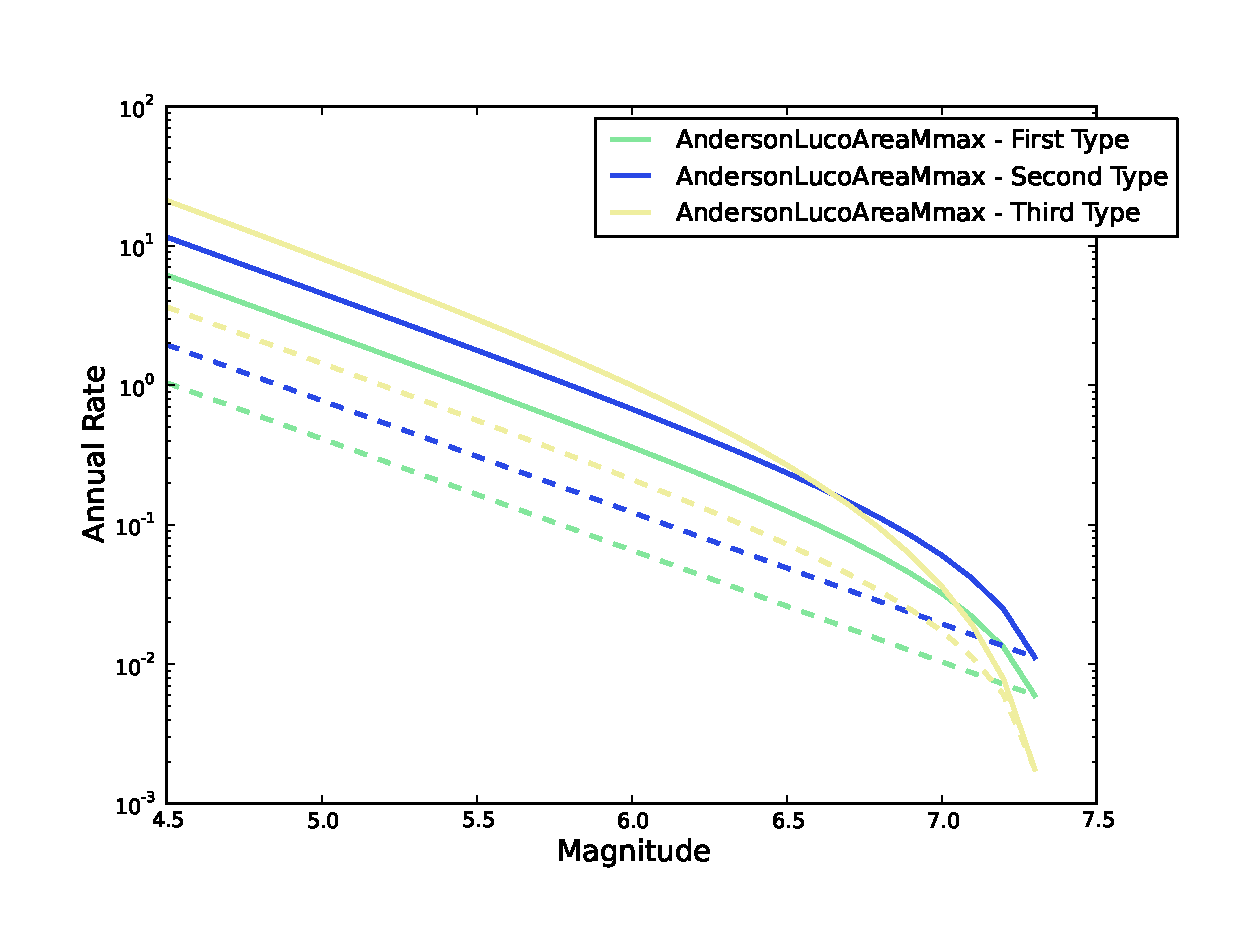
\includegraphics[trim=5mm 5mm 5mm 5mm, clip, width=12cm]{./figures/anderson_luco_mmax_mfds.eps}
  \caption{Comparison of magnitude frequency distributions for the specified fault using the three different models of the \textcite{AndersonLuco1983} ``Area-Mmax'' configuration}
  \label{fig:anderson_luco_area_mmax}
\end{figure}

The three distributions can compared visually for the same fault using the plotting tools shown previously. The example below, using the same fault properties defined previously, will generate a plot similar to that shown in Figure \ref{fig:anderson_luco_area_mmax}.

\begin{python}[frame=single]
>> and_luc_config1 = {'Model_Name': 'AndersonLucoAreaMmax',
                      'Model_Type': 'First',
                      'Model_Weight': 1.0,  
                      'MFD_spacing': 0.1,
                      'Maximum_Magnitude': None,
                      'Minimum_Magnitude': 4.5,
                      'b_value': [0.8, 0.05]}
>> and_luc_config2 = {'Model_Name': 'AndersonLucoAreaMmax',
                      'Model_Type': 'Second',
                      'Model_Weight': 1.0,
                      'MFD_spacing': 0.1,
                      'Maximum_Magnitude': None,
                      'Minimum_Magnitude': 4.5,
                      'b_value': [0.8, 0.05]}
>> and_luc_config3 = {'Model_Name': 'AndersonLucoAreaMmax',
                      'Model_Type': 'Third',
                      'Model_Weight': 1.0,   
                      'MFD_spacing': 0.1,
                      'Maximum_Magnitude': None,
                      'Minimum_Magnitude': 4.5,
                      'b_value': [0.8, 0.05]}
>> anderson_luco_area_mmax = [and_luc_config1,
                              and_luc_config2,
                              and_luc_config3]
>> plot_recurrence_models(anderson_luco_area_mmax,
                          area,
                          slip,
                          msr,
                          rake,
                          disp_length_ratio=1.25E-5, 
                          msr_sigma=0.0)

\end{python}

\subsubsection{Characteristic}

Although the term ``Characteristic'' may take on certain different meanings in the literature, in the present calculator it is referring to the circumstance when the fault is assumed to rupture with magnitudes distributed in a narrow range around the single characteristic magnitude. The model is therefore a truncated Gaussian distribution, in which the following must be specified: mean characteristic magnitude, the uncertainty (in magnitude units) and the number of standard deviations above and below the mean to be used as truncation limits.

\begin{Verbatim}[frame=single, commandchars=\\\{\}, fontsize=\scriptsize]
          \# Example of constructor for characteristic earthquake
        - Model_Type: Characteristic
          \# Spacing (magnitude units) of the magnitude frequency distribution
          MFD_spacing: 0.1
          \# Weight of the model
          Model_Weight: 0.2
          \# Magnitude of the Characteristic Earthquake
          Maximum_Magnitude:
          \# Uncertainty on Characteristic Magnitude (in magnitude units)
          Sigma: 0.12
          \# Lower bound truncation (in number of standard deviations)
          Lower_Bound: -3.0
          \# Upper bound truncation (in number of standard deviations)
          Upper_Bound: 3.0
\end{Verbatim}

The parameters \verb=Model_Type=, \verb= MFD_Spacing=, \verb=Model_Weight=, and\verb= Maximum_Magnitude= are as described for the previous calculators. \verb=Sigma= is the uncertainty of the characteristic magnitude (in magnitude units), and \verb=Lower_Bound= and \verb=Upper_Bound= are the lower and upper truncation limits of the Gaussian distribution respectively. Note that setting \verb=Sigma= to 0.0 or \verb=Lower_Bound= and \verb=Upper_Bound= to zero will simply result in the characteristic magnitude being evaluated as a single Dirac function.

\begin{figure}[htb]
  \centering
      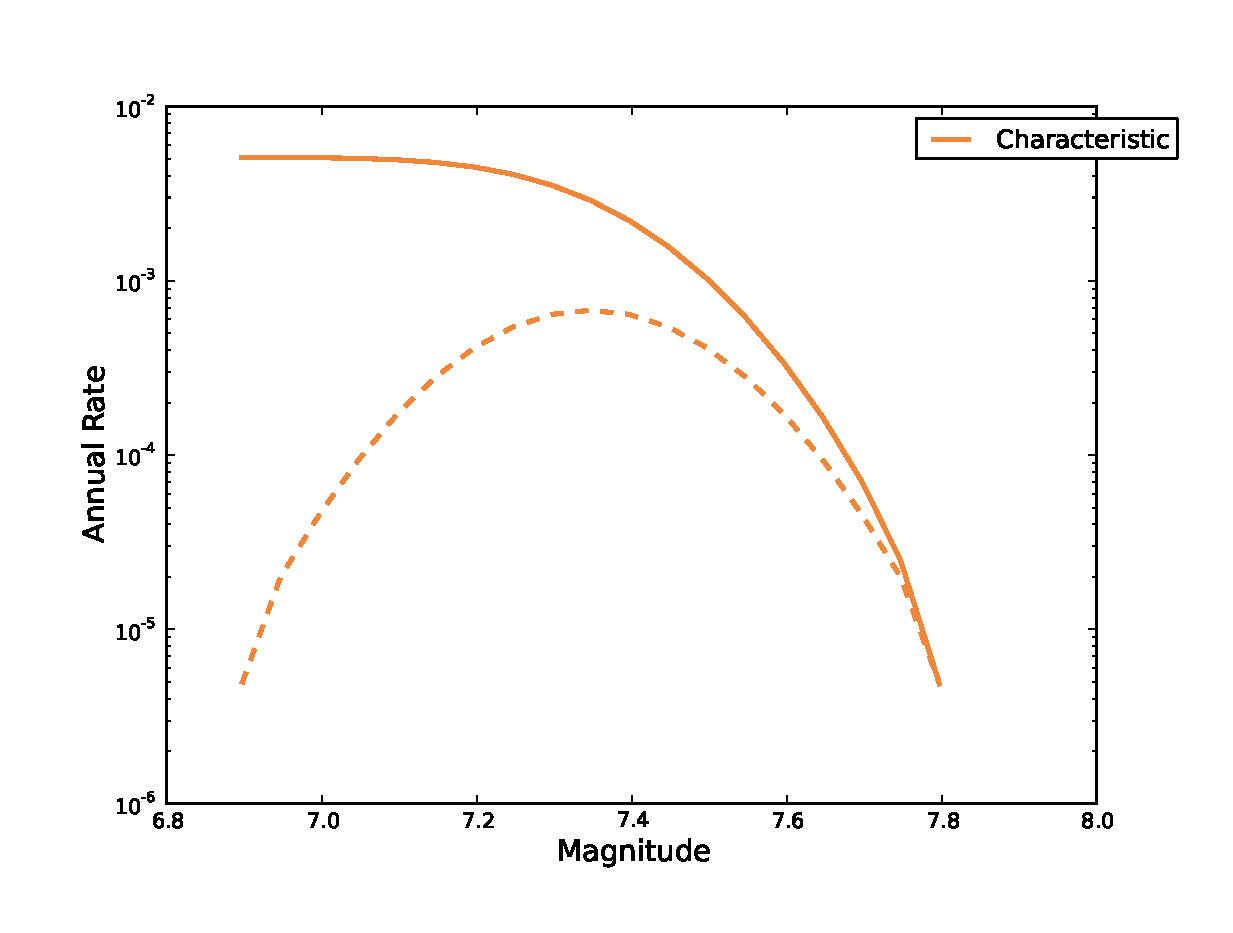
\includegraphics[trim=5mm 5mm 5mm 5mm, clip, width=12cm]{./figures/characteristic_mfds.eps}
  \caption{Magnitude frequency distribution for the specified fault configuration using the ``Characteristic'' model}
  \label{fig:characteristic}
\end{figure}

The distribution is shown, for the fault example defined previously, in Figure \ref{fig:characteristic}, which is generated using the code example shown below:

\begin{python}[frame=single]
>> characteristic = [{'Model_Name': 'Characteristic',
                      'MFD_spacing': 0.05,
                      'Model_Weight': 1.0,
                      'Maximum_Magnitude': None,
                      'Sigma': 0.15, 
                      'Lower_Bound': -3.0, 
                      'Upper_Bound': 3.0}]
>> plot_recurrence_models(characteristic,
                          area,
                          slip,
                          msr,
                          rake,
                          msr_sigma=0.0)
\end{python}                               

\subsubsection{\textcite{YoungsCoppersmith1985} ``Exponential''}

This model is another form of ``Exponential'' model and is noted as being similar in construct to the \textcite{AndersonLuco1983} Type 2 models. It is included here mostly for completeness. The model is given as:

\begin{equation}
N \left( {M_W \geq M} \right) = \frac{\mu A \dot{s} \left( {1.5 - b} \right) \left( {1 - \exp \left( {-\beta \left( {M_{MAX} - M} \right)} \right)} \right)}{b M_{0}^{MAX} \exp \left( {-\beta \left( {M_{MAX} - M} \right)} \right)}
\end{equation}
where $M_0^{MAX}$ is the moment corresponding to the maximum magnitude. The inputs for the model are defined in a similar manner as for the \textcite{AndersonLuco1983} models:

\begin{Verbatim}[frame=single, commandchars=\\\{\}, fontsize=\scriptsize]
        - Model_Name: YoungsCoppersmithExponential
          \# Example constructor of the Youngs & Coppersmith (1985) Exponential model
          MFD_spacing: 0.1
          Model_Weight: 0.3
          Maximum_Magnitude:
          Maximum_Magnitude_Uncertainty:
          Minimum_Magnitude: 5.0
          b_value: [0.8, 0.05]
\end{Verbatim}

Note that all of the exponential models described here contain the term $d - b$, or some variant thereof, where $d$ is equal to 1.5. This introduces the condition that $b \leq 1.5$. 

\subsubsection{\textcite{YoungsCoppersmith1985} ``Characteristic''}

The \textcite{YoungsCoppersmith1985} model is a hybrid model, comprising an exponential distribution for lower magnitudes and a fixed recurrence rate for the characteristic magnitude $M_C$. The exponential component of the model is described via:

\begin{equation}
N \left( M \right) - N \left( {M_C} \right) = \frac{\mu A \dot{s}\ e^{\left( {-\beta \left( {M_{MAX} - M - 0.5} \right)}\right)} M_{0}^{MAX}}{1 - e^{\left( {-\beta \left( {M_{MAX} - M - 0.5} \right)} \right)}} 
 \left[ {\frac{b10^{-c/2}}{c - b} + \frac{b e^{\beta}\left({1 - 10^{-c/2}}\right)}{c}} \right]\end{equation}

where $\beta = b \ln \left( {10} \right)$, $c = 1.5$ and all other parameters are described as for the \textcite{YoungsCoppersmith1985} ``Exponential'' and \textcite{AndersonLuco1983} models. The rate for the characteristic magnitude is then given by:

\begin{equation}
N \left( {M_C} \right) = \frac{\beta \left( {N \left( M \right) - N \left( {M_C} \right)} \right) e^{-\beta \left( {M_{MAX} - M - 1.5} \right)}}{2 \left( {1 - e^{-\beta \left( {M_{MAX} - M - 1.5} \right)}} \right)}
\end{equation}

As described in \textcite{YoungsCoppersmith1985}, this model assumes that:
\begin{enumerate}
\item The characteristic magnitude bin width $\Delta M_C$ is 0.5 $M_W$
\item Magnitudes are exponentially distributed up to a value $M'$, where $M' = M_{MAX} - \Delta M_C$
\item The absolute rate of characteristic earthquakes $\dot{M} \left( {M_C} \right)$ is approximately equal to $\dot{M} \left( {M' - 1} \right)$
\end{enumerate}

The current calculator adopts the implementation found in the \href{http://docs.openquake.org/oq-hazardlib/mfd.html#module-openquake.hazardlib.mfd.youngs_coppersmith_1985}{OpenQuake hazardlib}. At present, these three model assumptions are hard-coded, meaning that the distribution need only be defined from the moment rate and the characteristic magnitude. For [implementation] simplicity the input definition for the characteristic earthquake model is actually the same as for the exponential model. However, here the attribute \verb=Maximum_Magnitude= is actually referring to the characteristic magnitude and not to the absolute maximum magnitude, which will be 0.25 larger. 

\begin{figure}[htb]
  \centering
      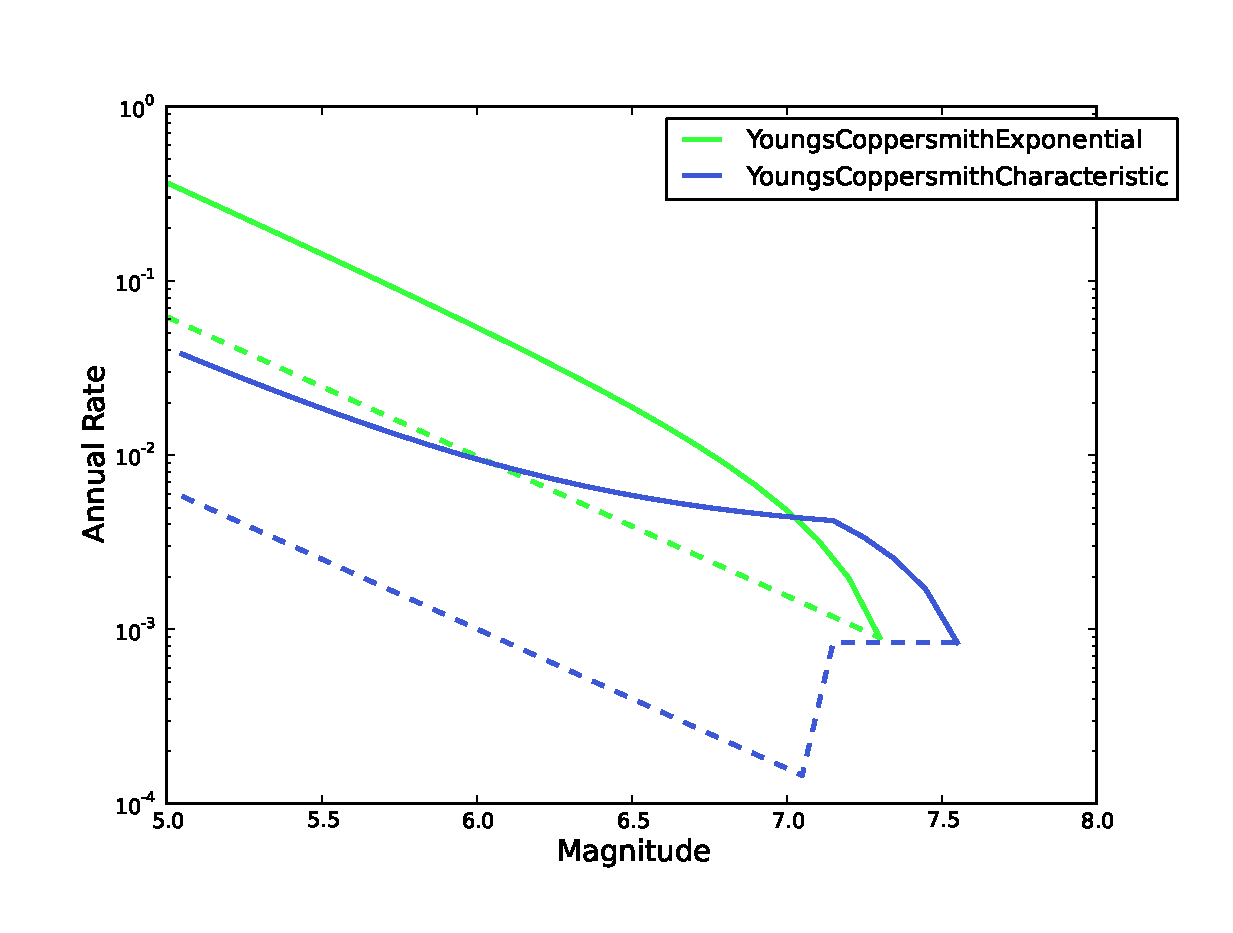
\includegraphics[trim=5mm 5mm 5mm 5mm, clip, width=12cm]{./figures/youngs_coppersmith_mfds.eps}
  \caption{Magnitude frequency distribution for the specified fault configuration using the \textcite{YoungsCoppersmith1985} ``Exponential'' and ``Hybrid'' models}
  \label{fig:youngs_coppersmith}
\end{figure}

The two \textcite{YoungsCoppersmith1985} distributions are compared in Figure \ref{fig:youngs_coppersmith}, which is generated using the code below:
\begin{python}[frame=single]
>> exponential = {'Model_Name': 'YoungsCoppersmithExponential',
                  'MFD_spacing': 0.1,
                  'Maximum_Magnitude': None,
                  'Maximum_Magnitude_Uncertainty': None,
                  'Minimum_Magnitude': 5.0,
                  'Model_Weight': 1.0,
                  'b_value': [0.8, 0.1]}

>> hybrid = {'Model_Name': 'YoungsCoppersmithCharacteristic',
             'MFD_spacing': 0.1,
             'Maximum_Magnitude': None,
             'Maximum_Magnitude_Uncertainty': None,
             'Minimum_Magnitude': 5.0,
             'Model_Weight': 1.0,
             'b_value': [0.8, 0.1],
             'delta_m': None}

>> youngs_coppersmith = [exponential, hybrid]

# View the corresponding magnitude recurrence model
>> plot_recurrence_models(youngs_coppersmith,
                          area,
                          slip,
                          msr,
                          rake,
                          msr_sigma=0.0)
\end{python}

\subsection{Running a Recurrence Calculation from Geology}

The particulars of the geological workflow are largely established in the input definition, and not in the configuration file. Execution of the whole process is then relatively simple, so it is broken down here into two steps. The first step simply imports an appropriate parser and loads the fault source. The parser contains a method called \verb=read_file(x)= which takes as an input the desired mesh spacing (in km) used to create the mesh of the fault surface. In the example below this is set to 1.0 km, but for large complex faults (such as large subduction zones) it may be desirable to select a larger spacing to avoid storing a large mesh in RAM.

\begin{python}[frame=single]
>> from hmtk.parsers.faults.fault_yaml_parser import\
    FaultYmltoSource

>> input_file = 'path/to/fault_model_file.yml'

>> parser = FaultYmltoSource(input_file)

# Spacing of the fault mesh (km) must be specified 
# at input (here 1.0 km) 
>> fault_model, tect_reg = parser.read_file(1.0)
\end{python}

In the second step, we simply execute the method to calculate the recurrence on the fault, and the write the resulting source model to an xml file. 

\begin{python}[frame=single]
# Builds the fault model
>> fault_model.build_fault_model()
# Specify the xml file for writing the output model
>> output_file  = 'path/to/output_source_model_file.yml'

>> fault_model.source_model.serialise_to_nrml(outfile,
                                              use_defaults=True)
\end{python}

The serialiser takes as an optional input the choice to accept default values for certain attributes that may be missing from the fault source definition. These values are as follows:

\begin{table}[h]
\begin{tabular}{|c|c|} \hline
\textbf{Attribute} & \textbf{Default Value} \\ \hline
Aspect Ratio & 1.0 \\
Magnitude Scaling Relation & \cite{wells1994} ('WC1994') \\
Nodal Plane Distribution & Strike = 0., Dip = 90, Rake = 0., probability= 1.0\\
Hypocentral Depth Distribution & Depth = 10.0 km, Probability = 1.0 \\ \hline

\end{tabular}

\end{table}

\subsubsection{Epistemic Uncertainties}

The following example compares the case when epistemic uncertainties are incorporated into the analysis. A demonstration file (\verb=tests/parsers/faults/yaml_examples/=\\
\verb=simple_fault_example_4branch.yml=) is included, which considers two epistemic uncertainties for a specific fault: slip rate and magnitude frequency distribution type. The fault has two estimates of slip rate (5 $mm \ yr^{-1}$ and 7 $mm\ yr^{-1}$), each assigned a weighting of 0.5. Two magnitude frequency distribution types (Characteristic and \textcite{AndersonLuco1983} ``Arbitrary'') are assigned, with weights of 0.7 and 0.3 respectively. The analysis is run, in the manner described previously. Firstly we consider the case when the different options are enumerated (the default option:

\begin{python}[frame=single]
>> from hmtk.parsers.faults.fault_yaml_parser import\
    FaultYmltoSource
>> input_file = \
 'tests/parsers/faults/yaml_examples/
  simple_fault_example_4branch.yml'
>> parser = FaultYmltoSource(input_file) 
>> fault_model, tect_reg = parser.read_file(1.0)
>> fault_model.build_fault_model()
>> output_file  = 'path/to/output_source_model_file.yml'
>> fault_model.source_model.serialise_to_nrml(output_file,
                                              use_defaults=True)
\end{python}

As four different activity rates are produced, the source is duplicated four time, each with an activity rate that corresponds to the rate calculated for the specific branch, multiplied by the weight of the branch. The output is a nrml file with four sources, as illustrated below:

\begin{Verbatim}[frame=single, commandchars=\\\{\}, fontsize=\scriptsize]
<?xml version='1.0' encoding='UTF-8'?>
<nrml xmlns:gml="http://www.opengis.net/gml" xmlns="http://openquake.org/xmlns/nrml/0.4">
  <sourceModel name="Template Simple Fault">
    <simpleFaultSource id="1_1" name="A Simple Fault" tectonicRegion="Active Shallow Crust">
      <simpleFaultGeometry>
        <gml:LineString>
          <gml:posList>30.0 30.0 30.0 31.0</gml:posList>
        </gml:LineString>
        <dip>30.0</dip>
        <upperSeismoDepth>0.0</upperSeismoDepth>
        <lowerSeismoDepth>20.0</lowerSeismoDepth>
      </simpleFaultGeometry>
      <magScaleRel>WC1994</magScaleRel>
      <ruptAspectRatio>1.5</ruptAspectRatio>
      <incrementalMFD minMag="6.64" binWidth="0.1">
        <occurRates>1.66984888376e-05 0.000165760464747 0.000658012622916 
                    0.00135343006814 0.00144508466725 0.00080109356265 
                    0.000230216031359 3.05523435745e-05 0.0</occurRates>
      </incrementalMFD>
      <rake>-90.0</rake>
    </simpleFaultSource>
    <simpleFaultSource id="1_2" name="A Simple Fault" tectonicRegion="Active Shallow Crust">
      <simpleFaultGeometry>
        <gml:LineString>
          <gml:posList>30.0 30.0 30.0 31.0</gml:posList>
        </gml:LineString>
        <dip>30.0</dip>
        <upperSeismoDepth>0.0</upperSeismoDepth>
        <lowerSeismoDepth>20.0</lowerSeismoDepth>
      </simpleFaultGeometry>
      <magScaleRel>WC1994</magScaleRel>
      <ruptAspectRatio>1.5</ruptAspectRatio>
      <incrementalMFD minMag="4.5" binWidth="0.1">
        <occurRates>0.0404671423911 0.033659102961 0.0279964224108 
                    0.0232864098818 0.0193687920987 0.0161102595577 
                    0.0133999302432 0.0111455765116 0.00927048675038
                    0.00771085501945 0.00641360984941 0.00533460831472
                    0.00443713392921 0.00369064724985 0.00306974667434
                    0.00255330407018 0.00212374582219 0.00176645483392
                    0.00146927313415 0.00122208816284 0.00101648865894
                    0.000845478440245 0.000703238335844 0.000584928170206
                    0.000486522060675 0.000404671423911</occurRates>
      </incrementalMFD>
      <rake>-90.0</rake>
    </simpleFaultSource>
    <simpleFaultSource id="1_3" name="A Simple Fault" tectonicRegion="Active Shallow Crust">
      <simpleFaultGeometry>
        <gml:LineString>
          <gml:posList>30.0 30.0 30.0 31.0</gml:posList>
        </gml:LineString>
        <dip>30.0</dip>
        <upperSeismoDepth>0.0</upperSeismoDepth>
        <lowerSeismoDepth>20.0</lowerSeismoDepth>
      </simpleFaultGeometry>
      <magScaleRel>WC1994</magScaleRel>
      <ruptAspectRatio>1.5</ruptAspectRatio>
      <incrementalMFD minMag="6.64" binWidth="0.1">
        <occurRates>2.33778843726e-05 0.000232064650645 0.000921217672083
                    0.0018948020954 0.00202311853414 0.00112153098771 
                    0.000322302443902 4.27732810043e-05 0.0</occurRates>
      </incrementalMFD>
      <rake>-90.0</rake>
    </simpleFaultSource>
    <simpleFaultSource id="1_4" name="A Simple Fault" tectonicRegion="Active Shallow Crust">
      <simpleFaultGeometry>
        <gml:LineString>
          <gml:posList>30.0 30.0 30.0 31.0</gml:posList>
        </gml:LineString>
        <dip>30.0</dip>
        <upperSeismoDepth>0.0</upperSeismoDepth>
        <lowerSeismoDepth>20.0</lowerSeismoDepth>
      </simpleFaultGeometry>
      <magScaleRel>WC1994</magScaleRel>
      <ruptAspectRatio>1.5</ruptAspectRatio>
      <incrementalMFD minMag="4.5" binWidth="0.1">
        <occurRates>0.0566539993476 0.0471227441454 0.0391949913751
                    0.0326009738345 0.0271163089382 0.0225543633808 
                    0.0187599023404 0.0156038071162 0.0129786814505
                    0.0107951970272 0.00897905378917 0.00746845164061
                    0.00621198750089 0.00516690614979 0.00429764534408
                    0.00357462569825 0.00297324415106 0.00247303676749
                    0.00205698238781 0.00171092342797 0.00142308412252
                    0.00118366981634 0.000984533670182 0.000818899438288
                    0.000681130884944 0.000566539993476</occurRates>
      </incrementalMFD>
      <rake>-90.0</rake>
    </simpleFaultSource>
  </sourceModel>
</nrml>
\end{Verbatim}

If, alternatively, the user wishes to collapse the logic tree branches to give a single source as an output, this option can be selected as follows:

\begin{python}[frame=single]
...
>> from openquake.hazardlib.scalerel.wc1994 import WC1994
>> fault_model.build_fault_model(collapse=True,
                                 rendered_msr=WC1994())
...
\end{python}

To collapse the branches it is simple necessary to specify as an input to the function \verb=collapse= \verb=True=. The second option requires further explanation. A seismogenic source requires the definition of a corresponding magnitude scaling relation, even if multiple scaling relations have been used as part of the epistemic uncertainty analysis. As collapsing the branches means that the activity rate is no longer associated with a specified scaling relation, but is an aggregate of many, the user must select the scaling relation to be associated with the output activity rate, for use in the OpenQuake hazard calculation. Therefore the input \verb=rendered_msr= must be given an instance of one of the supported magnitude scaling relationships.

The output file should resemble the following:

\begin{Verbatim}[frame=single, commandchars=\\\{\}, fontsize=\scriptsize]
<?xml version='1.0' encoding='UTF-8'?>
<nrml xmlns:gml="http://www.opengis.net/gml" xmlns="http://openquake.org/xmlns/nrml/0.4">
  <sourceModel name="Template Simple Fault">
    <simpleFaultSource id="1_1" name="A Simple Fault" tectonicRegion="Active Shallow Crust">
      <simpleFaultGeometry>
        <gml:LineString>
          <gml:posList>30.0 30.0 30.0 31.0</gml:posList>
        </gml:LineString>
        <dip>30.0</dip>
        <upperSeismoDepth>0.0</upperSeismoDepth>
        <lowerSeismoDepth>20.0</lowerSeismoDepth>
      </simpleFaultGeometry>
      <magScaleRel>WC1994</magScaleRel>
      <ruptAspectRatio>1.5</ruptAspectRatio>
      <incrementalMFD minMag="4.5" binWidth="0.1">
        <occurRates>0.0971211417387 0.0807818471064 0.0671914137858
                    0.0558873837162 0.0464851010369 0.0386646229385
                    0.0321598325836 0.0267493836278 0.0222491682009
                    0.0185060520467 0.0153926636386 0.0128030599553
                    0.0106491214301 0.00885755339963 0.00736739201842
                    0.00612792976843 0.00509698997324 0.00423949160142 
                    0.00352625552195 0.00293301159081 0.00243957278146
                    0.00202914825659 0.00184661595792 0.00231362389313
                    0.00360190992617 0.00434969292261 0.00243432469089
                    0.000909841780938 0.000164472079868 0.0</occurRates>
      </incrementalMFD>
      <rake>-90.0</rake>
    </simpleFaultSource>
  </sourceModel>
</nrml>
\end{Verbatim}

